\documentclass[12pt,a4paper]{article}

% -------------------
% MARK: Packages
% -------------------

% import geometry package to update the document margins
\usepackage[margin=1in]{geometry}
% set the font to helvectica
\usepackage[scaled]{helvet}
\renewcommand\familydefault{\sfdefault}
% for type-setting
\usepackage{amsmath, amssymb, amsfonts, verbatim, pifont}
% for slashed out text
\usepackage[normalem]{ulem}
% for units and scientific notation
\usepackage[table]{xcolor}
\usepackage{siunitx}
% for references and URLs
\usepackage{hyperref, url}
% Natbib setup for author-year style
\usepackage{natbib}
 \bibpunct[, ]{(}{)}{,}{a}{}{,}%
 \def\bibfont{\small}%
 \def\bibsep{\smallskipamount}%
 \def\bibhang{24pt}%
 \def\newblock{\ }%
 \def\BIBand{and}%
% for graphics and figures
\usepackage{graphicx, subfig, tikz}
% force figures to stay in their sections
\usepackage[section]{placeins}
% for tables
\usepackage{booktabs, longtable, tabularx}
\usepackage{multicol, multirow}
\usepackage{adjustbox}
\usepackage[flushleft]{threeparttable}
% a package for working with .csv data for tables
\usepackage{csvsimple}
% setup the algorithm package
% ruled: show bars around title and bar at bottom
% lined: show the line column on the left of the algorithm
% linesnumbered: print line numbers for each line
\usepackage[ruled,lined,linesnumbered]{algorithm2e}
\DontPrintSemicolon % don't print the semicolon that \; usually prints
% fix overfull hbox errors from oddities like using
% quotes (``foo'') and etc.
\usepackage{microtype}

% -------------------
% MARK: Debugging Packages
% -------------------

% import a debugging package to show the margin boxes
% \usepackage{showframe}

% -------------------
% MARK: Declarations
% -------------------

% setup captions for tables and figures
\captionsetup[table]{%
  labelfont={bf},
  name={Table},
  labelsep=colon,
  justification=raggedright,
  singlelinecheck=false}
\captionsetup[figure]{%
  labelfont={bf},
  name={Figure},
  labelsep=colon,
  justification=raggedright,
  singlelinecheck=false}
\captionsetup[algorithm2e]{%
  labelfont={bf},
  name={Figure},
  labelsep=colon,
  justification=raggedright,
  singlelinecheck=false}

% set the graphics path to the img directory
\graphicspath{{img/}}

% -----------------------------------------------------------------------------
% MARK: algorithm2e stuff
% -----------------------------------------------------------------------------

% params
% \SetKwInOut{Objects}{$\CKmatrix{O}$}
% \SetKwInOut{Weights}{$\CKvector{w}$}

% -------------------
% MARK: Headers
% -------------------

% headers and footers
\usepackage{fancyhdr}
\setlength{\headheight}{15pt}
\pagestyle{fancy}
\lhead{KautenjaDSP}
\rhead{\itshape 2A03 v1.4.0}
\cfoot{\thepage}

% start the document
\begin{document}

% -------------------
% MARK: Title Page
% -------------------

% fancyhdr directive to remove headers from this title page
\thispagestyle{empty}
% center the title page contents
\vspace*{\fill}
\begin{center}

\includegraphics{2A03-Logo}
\linebreak\linebreak\linebreak\linebreak
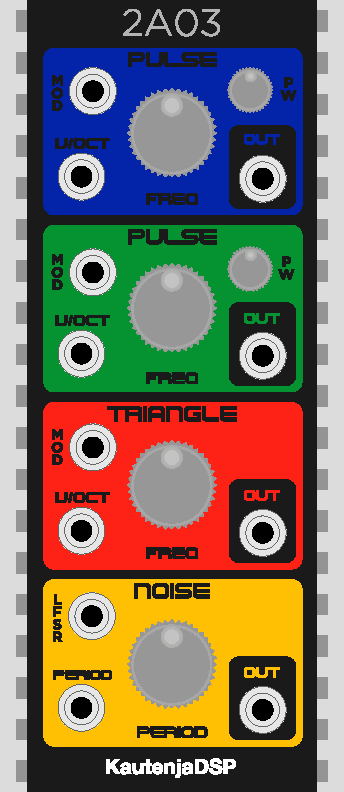
\includegraphics{2A03-Module}
\linebreak\linebreak\linebreak\linebreak

\includegraphics{KautenjaDSP}
\end{center}
\vspace*{\fill}
\clearpage

% -------------------
% MARK: Overview
% -------------------

\section{Overview}

2A03 is an emulation of the 2A03 sound chip from the Nintendo Entertainment System (NES) for VCV Rack. The 2A03 chip contains two pulse wave generators, a quantized triangle wave generator, and a noise generator. The original chip featured a DMC loader for playing samples that has been omitted in this emulation.

2A03 provides the key features of the 2A03 chip, namely,
\begin{itemize}
  \item \textbf{Dual pulse wave generator:} Dual 8-bit pulse waves with four duty cycles: $12.5\%$, $25\%$, $50\%$, and $75\%$;
  \item \textbf{Quantized triangle wave generator:} Generate NES style triangle wave with 16 steps of quantization;
  \item \textbf{Noise generator:} generate pseudo-random numbers at 16 different frequencies; and
  \item \textbf{Linear Feedback Shift Register (LFSR):} for that old-school 8-bit randomness!
\end{itemize}

% -------------------
% MARK: Panel Layout
% -------------------

\section{Panel Layout}

\begin{center}
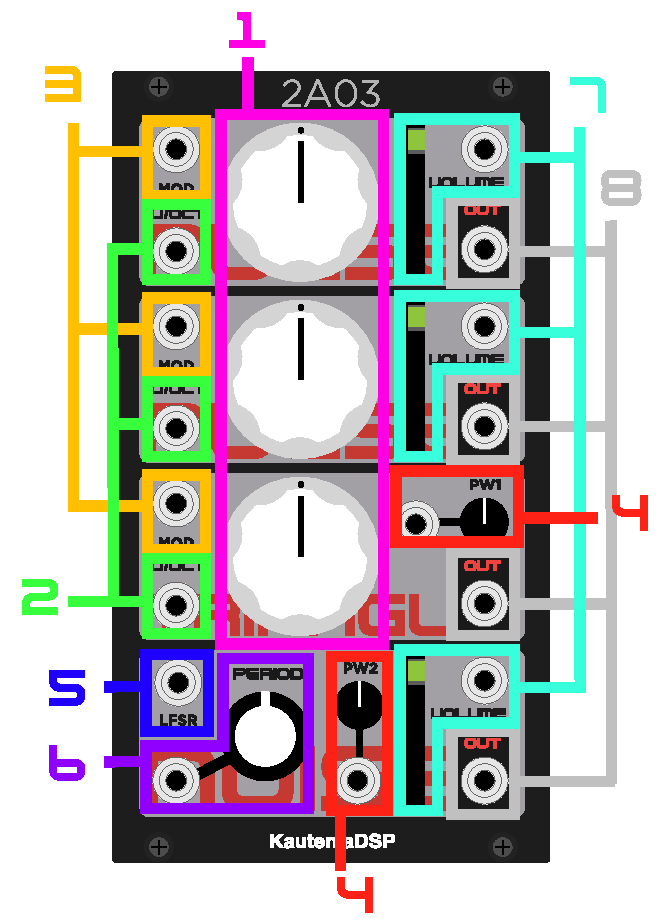
\includegraphics{2A03-Manual}
\end{center}

\begin{enumerate}
  \item Coarse frequency control over the four channels.
  \item $V$/Octave inputs for pulse1, pulse2, and triangle waveform generators.
  \item linear CV frequency modulation for pulse1, pulse2, and triangle waveform generators.
  \item Pulse width selector. Chooses between four duty cycles: $12.5\%$, $25\%$, $50\%$, and $75\%$.
  \item CV LFSR gate, high at $2V$. Holds the LFSR generator as long as the input voltage is $>2V$.
  \item Period of randomness $\in [0, 15]$ for the noise generator. See Table~\ref{tab:noise-periods} for a mapping from period to sample rate, frequency, and MIDI note.
  \item Coarse amplitude control over the channels using the 4-bit amplifier. When no input is connected, the slider controls the level from $0\%$ to $100\%$. When an input is connected, the slider acts as an attenuator.
  \item Channel outputs, ${\approx}10V_{pp}$.
\end{enumerate}

\begin{table}[!htp]
\centering
\caption{Mapping of noise period to sample rate, fundamental frequency, and MIDI note.}
\label{tab:noise-periods}
\begin{tabular}{|l||r|r|r|}
\hline
 Period  & Sample rate   & Fundamental   & MIDI note \\
\hline\hline
 0       & $447443.2 Hz$ & $4811.2 Hz$   & 110.41    \\
 1       & $223721.6 Hz$ & $2405.6 Hz$   & 98.41     \\
 2       & $111860.8 Hz$ & $1202.8 Hz$   & 86.41     \\
 3       & $55930.4 Hz$  & $601.4 Hz$    & 74.41     \\
 4       & $27965.2 Hz$  & $300.7 Hz$    & 62.41     \\
 5       & $18643.5 Hz$  & $200.5 Hz$    & 55.39     \\
 6       & $13982.6 Hz$  & $150.4 Hz$    & 50.41     \\
 7       & $11186.1 Hz$  & $120.3 Hz$    & 46.55     \\
 8       & $8860.3 Hz$   & $95.3 Hz$     & 42.51     \\
 9       & $7046.3 Hz$   & $75.8 Hz$     & 38.55     \\
 10      & $4709.9 Hz$   & $50.6 Hz$     & 31.57     \\
 11      & $3523.2 Hz$   & $37.9 Hz$     & 26.55     \\
 12      & $2348.8 Hz$   & $25.3 Hz$     & 19.53     \\
 13      & $1761.6 Hz$   & $18.9 Hz$     & 14.55     \\
 14      & $879.9 Hz$    & $9.5 Hz$      & 2.53      \\
 15      & $440.0 Hz$    & $4.7 Hz$      & -9.47     \\
\hline
\end{tabular}
\end{table}

% -------------------
% MARK: References
% -------------------

\clearpage
\renewcommand\refname{References \& Acknowledgments}
\nocite{*}
\bibliographystyle{apalike}
\bibliography{references}

\end{document}
